% !TEX encoding = UTF-8
% !TEX program = lualatex
% Page Layout
\documentclass{beamer}
%\documentclass[beamer]
\usepackage{amssymb}

\let\Tiny=\tiny
\usepackage{tikz}
\usetikzlibrary{decorations.text}

\usepackage{chemfig}
\usepackage{siunitx}
\usepackage{graphicx}
\usepackage{url}
\usepackage[german]{babel}
\usepackage[export]{adjustbox}
\usepackage{caption}
\usepackage{multirow}
\usepackage[T1]{fontenc}
\usepackage{fontspec,microtype}
\defaultfontfeatures{Ligatures=TeX, Scale=MatchLowercase}
\usepackage[german=quotes]{csquotes}
\setmainfont[SmallCapsFeatures={LetterSpace=6}, Numbers={Proportional,OldStyle}]{Minion Pro}
\setsansfont[LetterSpace=2, Numbers={Proportional,OldStyle}]{Myriad Pro}

\usepackage{array} % needed for \arraybackslash
\usepackage{tabularx}

\sisetup{
  round-mode          = places,
  round-precision     = 2,
  inter-unit-product =\ensuremath{{}\cdot{}}
}
 % Avoid an error due to a lack of registers

\definecolor{orange}{RGB}{255,127,0}
%\include{head}
\title[]{Alkaloiden}
\author[N. Arslan]{Nevroz Arslan}
\date[18.04.17]{18. Apr 2017}
%\titlegraphic{\includegraphics[width=\textwidth,height=.5\textheight]{bogen1200.png}}
\setbeamerfont{page number in head/foot}{size=\large}
\beamertemplatenavigationsymbolsempty


\let\otp\titlepage
\renewcommand{\titlepage}{\otp\addtocounter{framenumber}{-1}}

\renewcommand*\printatom[1]{\ensuremath{\mathsf{#1}}}


\definecolor{mygray}{RGB}{208,208,208}
\definecolor{mymagenta}{RGB}{226,0,116}
\newcommand*{\mytextstyle}{\sffamily\tiny\bfseries\color{black!85}}
\newcommand{\arcarrow}[3]{%
   % inner radius, middle radius, outer radius, start angle,
   % end angle, tip protusion angle, options, text
   \pgfmathsetmacro{\rin}{1.2}
   \pgfmathsetmacro{\rmid}{1.7}
   \pgfmathsetmacro{\rout}{2.2}
   \pgfmathsetmacro{\astart}{#1}
   \pgfmathsetmacro{\aend}{#2}
   \pgfmathsetmacro{\atip}{1}
   \fill[mygray, very thick] (\astart+\atip:\rin)
                         arc (\astart+\atip:\aend:\rin)
      -- (\aend-\atip:\rmid)
      -- (\aend:\rout)   arc (\aend:\astart+\atip:\rout)
      -- (\astart:\rmid) -- cycle;
   \path[
      decoration = {
         text along path,
         text = {|\mytextstyle|#3},
         text align = {align = center},
         raise = -1.0ex
      },
      decorate
   ](\astart+\atip:\rmid) arc (\astart+\atip:\aend+\atip:\rmid);
}

\newcommand{\arckarrow}[3]{%
   % inner radius, middle radius, outer radius, start angle,
   % end angle, tip protusion angle, options, text
   \pgfmathsetmacro{\rin}{1.2}
   \pgfmathsetmacro{\rmid}{1.7}
   \pgfmathsetmacro{\rout}{2.2}
   \pgfmathsetmacro{\astart}{#1}
   \pgfmathsetmacro{\aend}{#2}
   \pgfmathsetmacro{\atip}{1}
   \fill[mygray, very thick] (\astart+\atip:\rin)
                         arc (\astart+\atip:\aend:\rin)
      -- (\aend-\atip:\rmid)
      -- (\aend:\rout)   arc (\aend:\astart+\atip:\rout)
      -- (\astart:\rmid) -- cycle;
   \path[
      decoration = {
         text along path,
         text = {|\mytextstyle|#3},
         text align = {align = center},
         raise = -1.0ex,
         reverse path
      },
      decorate
   ](\astart+\atip:\rmid) arc (\astart+\atip:\aend+\atip:\rmid);
}


\newcommand{\arcyarrow}[3]{%
   % inner radius, middle radius, outer radius, start angle,
   % end angle, tip protusion angle, options, text
   \pgfmathsetmacro{\rin}{2.3}
   \pgfmathsetmacro{\rmid}{2.8}
   \pgfmathsetmacro{\rout}{3.2}
   \pgfmathsetmacro{\astart}{#1}
   \pgfmathsetmacro{\aend}{#2}
   \pgfmathsetmacro{\atip}{1}
   \fill[mygray, very thick] (\astart+\atip:\rin)
                         arc (\astart+\atip:\aend:\rin)
      -- (\aend-\atip:\rmid)
      -- (\aend:\rout)   arc (\aend:\astart+\atip:\rout)
      -- (\astart:\rmid) -- cycle;
   \path[
      decoration = {
         text along path,
         text = {|\mytextstyle|#3},
         text align = {align = center},
         raise = -1.0ex,
      },
      decorate
   ](\astart+\atip:\rmid) arc (\astart+\atip:\aend+\atip:\rmid);
}

\newcommand{\arcyrarrow}[3]{%
   % inner radius, middle radius, outer radius, start angle,
   % end angle, tip protusion angle, options, text
   \pgfmathsetmacro{\rin}{2.3}
   \pgfmathsetmacro{\rmid}{2.8}
   \pgfmathsetmacro{\rout}{3.2}
   \pgfmathsetmacro{\astart}{#1}
   \pgfmathsetmacro{\aend}{#2}
   \pgfmathsetmacro{\atip}{1}
   \fill[mygray, very thick] (\astart+\atip:\rin)
                         arc (\astart+\atip:\aend:\rin)
      -- (\aend-\atip:\rmid)
      -- (\aend:\rout)   arc (\aend:\astart+\atip:\rout)
      -- (\astart:\rmid) -- cycle;
   \path[
      decoration = {
         text along path,
         text = {|\mytextstyle|#3},
         text align = {align = center},
         raise = -1.0ex,
         reverse path
      },
      decorate
   ](\astart+\atip:\rmid) arc (\astart+\atip:\aend+\atip:\rmid);
}



\begin{document}
\makeatletter
\newenvironment{myitemize}{%
   \setlength{\topsep}{0pt}
   \setlength{\partopsep}{0pt}
   \renewcommand*{\@listi}{\leftmargin\leftmargini \parsep\z@ \topsep\z@ \itemsep\z@}
   \let\@listI\@listi
   \itemize
}{\enditemize}
\makeatother   


\setbeamercolor{block title}{use=structure,fg=black,bg=white}
\setbeamercolor{block body}{use=structure,fg=black,bg=white}
\setbeamerfont{frametitle}{size=\large}
\usebackgroundtemplate{
\includegraphics[width=1.0\paperwidth,height=0.17\paperheight]{bogen1200}
\begin{tikzpicture}[overlay, remember picture]
    \node[xshift=-10.80cm,yshift=1.15cm] at (0,0)    {\includegraphics[scale=0.6]{logo}};
\end{tikzpicture}
}


\addtobeamertemplate{frametitle}{\vskip+7ex}{}
\setbeamercolor{frametitle}{fg=black}
\setbeamertemplate{caption}{\insertcaption}

\setbeamertemplate{itemize/enumerate body begin}{\normalsize}
\setbeamerfont{frametitle}{size=\large}
\frame[plain]{\titlepage}
\defbeamertemplate{footline}{centered page number}
{%
 \hfill%
  \usebeamercolor[fg]{page number in head/foot}%
  \usebeamerfont{page number in head/foot}%
  \raisebox{.5cm}[0pt][0pt]{% <--- change here
    \insertframenumber\,/\,\inserttotalframenumber\kern1em}%
}

\setbeamertemplate{footline}[centered page number]
\setatomsep{3em}
\setdoublesep{4pt}

% tikz macro





\begin{frame}[t]{title}
 
\begin{tikzpicture}
  \colorlet{good}{green!75!black}
  \colorlet{bad}{red}
  \colorlet{neutral}{black!60}
  \colorlet{none}{white}

  \node[align=center,text width=2cm]{Photosynthese};
\draw[step=.5cm,gray,very thin] (-3,-2) grid (3,4);
%  \begin{scope}[line width=4mm]
%    \draw[good] (-250:2cm) arc (-250:-270:2cm);
    %\draw[good!60!white] (-36:2cm) arc (-36:-101:2cm);
    %\draw[neutral]       (-36:2cm) arc (-36:36:2cm);
    %\draw[bad!60!white]  (36:2cm)  arc (36:93:2cm);

%    \newcount\mycount
%    \foreach \angle in {0,72,...,3599}
%    {
%      \mycount=\angle\relax
%      \divide\mycount by 10\relax
%      \draw[black!15,thick] (\the\mycount:18mm) -- (\the\mycount:22mm);
%    }

 %   \draw (0:2.2cm) node[below] {Alkaloide};
 %   \draw (165:2.2cm) node[above] {};
 %   \draw (-111:2.2cm) node[left] {};
 %   \draw (-68:2.2cm) node[left] {};
 %   \draw (65:2.2cm) node[right] {};
 %   \draw (93:2.2cm) node[right] {};
 % \end{scope}
  \draw[gray] (0,1) circle (3cm) circle (2cm) circle (1 cm);
  \draw (0,0) -- (0,-1);
\end{tikzpicture}

\end{frame}



\begin{frame}[t]{Alkaloiden - Klassifizierung}
\begin{quote}
  Die \enquote{echten} Alkaloide werden nach den in ihnen enthaltenen
  heterocyclischen Ringsystemen eingeteilt.
\end{quote}
  \begin{table}[htpb]
    \tiny
    %\caption{Wichtige Gruppen der Alkaloide mit Aminosäurenvorstufen}
    \begin{tabular}{llll}
      \hline
      Strukturgruppe & Alkaloid Gruppe & Vorstufe & Beispiele \\
      \hline
      \chemfig[][scale=0.5]{
        =^[:270]% 2
        -[:330]% 3
        =^[:30]% 4
        -[:90]% 5
        (
        =^[:150]% 6
        -[:210]% -> 1
        )
        -[:30]% 7
        =_[:330]% 8
        -[:270]% 9
        =_[:210]N% 10
        (
        -[:150]% -> 4
        )
      }& Chinolin & Tryptophan & Chinin \\
      \multirow{3}{*}{\chemfig[][scale=0.5]{
        -[:300.8]N% 2
        -[:279.7]% 3
        -[:233.9,1.069]% 4
        -[:31.3,0.88]% 5
        -[:65.7,0.943]% 6
        (
        -[:141.9,0.864]\phantom{N}% -> 2
        )
        -[:1,1.126]% 7
        -[:279.6,1.005]% 8
        (
        -[:30,,,1]OH% 10
        )
        -[:140.3,0.813]% 9
        (
        -[:180,1.178]% -> 3
        )
    } } &  &  & Cocain \\
        & Tropan & Ornithin& Scopolamin\\
        && & Hyoscyamin\\
        &&&\\
        &&&\\
   \multirow{4}{*}{\chemfig[][scale=0.5]{
        R=[:0]% 6
       -[:300]% 5
       =^[:0]% 4
                 (
           -[:300]% 34
                     (
            -[:0,,,1]OH% 36
                     )
           =[:240]O% 35
                 )
    -[:60,,,1]NH% 3
    -[:120,,1]% 2
                 (
           -[:180]% 1
           -[:240]% -> 6
                 )
        <[:60]% 37
                 (
           =[:120]O% 38
                 )
    -[:0,,,1]OH% 39
    } } & Betalaine & Tyrosin & Betanidin \\
        && & Indicaxanthin\\
        &&&\\
        &&&\\
        &&&\\
        &&&\\
\multirow{4}{*}{\chemfig[][scale=0.5]{
    =^[:270]% 2
     -[:330]% 3
     =^[:30]% 4
      -[:90]% 5
               (
        =^[:150]% 6
         -[:210]% -> 1
               )
      -[:18]% 7
    =_[:306]% 8
     -[:234]\chembelow{N}{H}% 9
               (
         -[:162]% -> 4
               )
    } } & Indol & Tryptophan & Harmin \\
        && & Ergolin\\
        && & Strychinin\\
        && & Reserpin
    \end{tabular}
  \end{table}

\end{frame}
\begin{frame}[t]{Alkaloide - Klassifizierung}
   \begin{table}[htpb]
    \tiny
  %  \caption{Wichtige Gruppen der Alkaloide - II}
    \begin{tabular}{llll}
      \hline
      Strukturgruppe & Alkaloid Gruppe & Vorstufe & Beispiele \\
      \hline
      \multirow{3}{*}{\chemfig[][scale=0.5]{
    =^[:270]% 2
     -[:330]% 3
     =^[:30]% 4
     -[:330]% 5
     =^[:30]N% 6
      -[:90]% 7
    =^[:150]% 8
     -[:210]% 9
               (
         -[:270]% -> 4
               )
    =^[:150]% 10
               (
         -[:210]% -> 1
               ) 
    } } & Isochinolin & Tyrosin & Morphin \\
        && & Codein\\
        && & Papaverin\\
   \chemfig[][scale=0.5]{
       =^[:180]% 2
     -[:240]% 3
    =^[:300]N% 4
           -% 5
     =^[:60]% 6
               (
         -[:120]% -> 1
               )
    }  & Pyridin & Ornithin & Nicotin \\
\multirow{4}{*}{\chemfig[][scale=0.5]{
     =_[:330]% 2
     -[:270]% 3
               (
         -[:342]N% 7
         =^[:54]% 8
         -[:126]\chemabove{N}{H}% 9
         -[:198]% -> 2
               )
    =_[:210]N% 4
     -[:150]% 5
     =_[:90]N% 6
               (
          -[:30]% -> 1
               )
    } } & Purin & Glycin & Adenin \\
        && & Guanin\\
        && & Theobromin\\
        && & Coffein
    \end{tabular}
  \end{table}

 
\end{frame}
  \begin{frame}[t]{Alkaloide - weitere Einteilung}
    \begin{quote}
      Angehörige einer dieser Alkaloidgruppen können weiter nach am genannten
      Ringsystem ankondensierten zusätzlichen Ringen bestimmten Typen zuordnen.  
    \end{quote}
  \begin{table}[htpb]
    \tiny
  %  \caption{Wichtige Gruppen der Alkaloide - II}
    \begin{tabular}{llll}
      \hline
      Gerüßt & Alkaloid & Typ & Zusatzfunktionen \\
      \hline
      \chemfig[][scale=0.5]{
          -[:270]% 2
       >[:330]% 3
        -[:30]% 4
                 (
        -[:90,,,1]NH% 15
        -[:150,,1]% 16
           -[:210]% -> 1
                 )
      <:[:330]% 5
       -[:270]% 6
    =_[:308.5]% 7
       -[:240]\chembelow{N}{H}% 8
     -[:171.5]% 9
      =_[:210]% 10
       -[:150]% 11
       =_[:90]% 12
        -[:30]% 13
                 (
            -[:90]% -> 3
                 )
      =_[:330]% 14
                 (
            -[:30]% -> 6
                 )
                 (
           -[:270]% -> 9
                 ) 
      }  & Ergolin & Ergolin & Isopren-Einheit, Methyl \\
   \chemfig[][scale=0.5]{
              -[:30]% 2
       >:[:330]% 3
        -[:270]% 4
        >[:330]% 5
         -[:30]% 6
        >:[:90]% 7
        -[:150]% 8
                  (
            -[:210]% -> 3
                  )
      <:[:98.6]N% 9
                  (
    -[:230.2,2.036]% 10
    -[:315.5,2.036]% -> 5
                  )
       -[:47.1]% 11
      -[:355.7]% 12
      -[:304.3]% 13
     =^[:252.9]% 14
                  (
          -[:201.4]% -> 7
                  )
      -[:324.9]\chembelow{N}{H}% 15
       -[:36.9]% 16
     =^[:108.9]% 17
                  (
          -[:180.9]% -> 13
                  )
       -[:48.9]% 18
     =_[:348.9]% 19
                  (
           -[:48.9]O% 22
          -[:348.9]% 23
                  )
      -[:288.9]% 20
     =_[:228.9]% 21
                  (
          -[:168.9]% -> 16
                  )    
      }  & Ibogain & Iboga & Monoterpen-Einheit, Alkoxy \\
       \chemfig[][scale=0.5]{
                  O% 12
           =[:210]% 11
           -[:150]% 10
           -[:210]% 9
         <[:135.7]O% 8
         -[:187.8]% 7
           -[:240]% 6
        =^[:292.2]% 5
    -[:280.1,1.91]% 4
      -[:333,1.91]N% 3
           -[:354]% 2
            -[:66]% 1
           >[:138]% 19
           -[:210]% 18
                     (
               -[:282]\phantom{N}% -> 3
                     )
           <[:150]% 17
            >[:90]% 16
                     (
             -[:164.3]% -> 5
                     )
            -[:30]% 15
                     (
                -[:90]% -> 9
                     )
           <[:330]% 14
                     (
               -[:270]% -> 19
                     )
           <:[:30]N% 13
                     (
                -[:90]% -> 11
                     )
         -[:308.5]% 25
                =_% 24
           -[:300]% 23
          =_[:240]% 22
           -[:180]% 21
          =_[:120]% 20
                     (
             -[:171.5]% -> 19
                     )
                     (
                -[:60]% -> 25
                     )
       }  & Strychnin & Strychnin & Secoiridoid monoterpene \\
   
    \end{tabular}

  \end{table}
 


  \end{frame}





\begin{frame}[t]{Capsaicin}
  
\chemfig[][scale=0.5]{
     -[:270]% 2
               (
         -[:330]% 3
               )
     -[:210]% 4
     =[:150]% 5
     -[:210]% 6
     -[:150]% 7
     -[:210]% 8
     -[:150]% 9
     -[:210]% 10
               (
         =[:270]O% 11
               )
     -[:150]\chemabove{N}{H}% 12
     -[:210]% 13
     -[:150]% 14
    =_[:210]% 15
     -[:150]% 16
               (
         -[:210]O% 21
         -[:270]% 22
               )
     =_[:90]% 17
               (
     -[:150,,,2]HO% 20
               )
      -[:30]% 18
    =_[:330]% 19
               (
         -[:270]% -> 14
       )}
       \begin{itemize}
         \item Capsaicinoide sind farblos und sehr stabil. 
         \item Capsaicin bindet an den TRP-Kanal TRPV1, der auch durch eine Erhöhung der Temperatur aktiviert wird. Von diesem Umstand leitet sich der Ausdruck „brennen“ ab.
       \end{itemize}
       \url{https://de.wikipedia.org/wiki/Capsaicin}
\end{frame}

\begin{frame}[t,label=mohn]{Mohngewächse - Papaver - Isochinoilin Alkaloide }
  \begin{columns}[onlytextwidth,t]
    \begin{column}{0.6\textwidth}
      \begin{minipage}[c][0.9\textheight][l]{\linewidth}
        \includegraphics[height=3cm]{data/mohn/saft}% Place your graphic here
      \end{minipage}
    \end{column}
    \begin{column}{0.4\textwidth}
      \begin{minipage}[c][0.9\textheight][l]{\linewidth}
        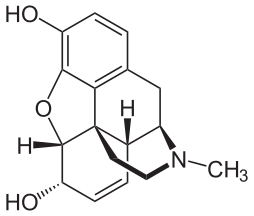
\includegraphics[height=3cm]{data/mohn/morphine}% Place your graphic here
      \end{minipage}
    \end{column}
  \end{columns}
\end{frame}
\begin{frame}[t,label=schoellkraut]{Mohngewächse - Schöllkraut - Spartein }
  \begin{columns}[onlytextwidth,t]
    \begin{column}{0.6\textwidth}
      \begin{minipage}[c][0.9\textheight][l]{\linewidth}
        \includegraphics[height=3cm]{data/mohn/schoellkraut}% Place your graphic here
      \end{minipage}
    \end{column}
    \begin{column}{0.4\textwidth}
      \begin{minipage}[c][0.9\textheight][l]{\linewidth}
        \begin{itemize}
          \item dies und das 
        \end{itemize}   
      \end{minipage}
    \end{column}
  \end{columns}


\end{frame}

%\definesubmol{&}{-[,,,,draw=none]}
%\begin{frame}[t,label=tryptamin]
  \frametitle{Tryptamin}
  \schemestart
  \chemfig[][scale=0.35]{
    O% 13
    =[:282]% 12
    (
    -[:342,,,1]OH% 14
    )
    -[:222]% 11
    (
    <[:282,,,1]NH_2% 15
    )
    -[:162]% 10
    -[:222]% 7
    -[:168]% 5
    -[:240]% 4
    (
    -[:312]\chembelow{N}{H}% 9
    -[:24]% 8
    =^[:96]% -> 7
    )
    =_[:180]% 3
    -[:120]% 2
    =_[:60]% 1
    -% 6
    (
    =_[:300]% -> 5
    )
  }
  \arrow
  \chemfig[][scale=0.35]{
              NH_2% 12
    -[:222,,1]% 11
       -[:162]% 10
       -[:222]% 7
       -[:168]% 5
       -[:240]% 4
                 (
           -[:312]\chembelow{N}{H}% 9
            -[:24]% 8
           =^[:96]% -> 7
                 )
      =_[:180]% 3
       -[:120]% 2
       =_[:60]% 1
             -% 6
                 (
          =_[:300]% -> 5
                 )
}
  \schemestop
\end{frame}



%\begin{frame}[t,label=ephedraarten]
  \frametitle{Ephedra Arten}
  \begin{table}[htpb]
  %  \caption{caption}
    \begin{tabular}{cc}
      Ephedra monosperma & adsda  \\ 
    \end{tabular}
  \end{table}
\end{frame}



%\begin{frame}[t]
  \frametitle{Pseudoephedrin}
  \begin{itemize}
    \item Pseudoephedrin bewirkt vorwiegend in der Körperperipherie eine Ausschüttung von Katecholaminen \footnotemark 
    \item indirektes Sympathomimetikum
    \item Pseudoephedrin ist ein Phenylethylamin-Alkaloid 
    \item \chemfig[][scale=0.35]{*6(-=-(-(<:[2]OH)-[:-30](<:[6]CH_3)-[:30]N-[:-30])=-=)}
 
  \end{itemize}
  \footnotetext{\url{https://de.wikipedia.org/wiki/Pseudoephedrin}}
\end{frame}





\end{document}
